\documentclass[11pt]{article}
\usepackage [colon,square]{natbib}
\usepackage[mathlines]{lineno} %% <- mathlines turns on line numbering in equations
\usepackage{amsmath}
\usepackage{printlen}
\setlength{\parindent}{10pt}
\setlength{\parskip}{10pt}
\usepackage[explicit]{titlesec}
\usepackage{helvet}
\usepackage{array}
\usepackage{printlen}
\usepackage[a4paper, margin=1.3cm]{geometry}
\usepackage{color,hyperref}
\catcode`\_=11\relax
\newcommand\email[1]{\_email #1\q_nil}
\def\_email#1@#2\q_nil{%
  \href{mailto:#1@#2}{{\emailfont #1\emailampersat #2}}
}
\newcommand\emailfont{\sffamily}
\newcommand\emailampersat{{\color{red}\small@}}
\catcode`\_=8\relax

\usepackage{hyperref}
\usepackage[export]{adjustbox}
\usepackage{bibentry}
\renewcommand{\bibfont}{\footnotesize}
\usepackage{tikz}
\usepackage{setspace}
\usepackage[inline,shortlabels]{enumitem}
\usepackage[all]{nowidow}
\def\checkmark{\tikz\fill[scale=0.4](0,.35) -- (.25,0) -- (1,.7) -- (.25,.15) -- cycle;}
\pagenumbering{gobble}
\hypersetup{ % Remove ugly boxes around URLs
  colorlinks, linkcolor={black!100!black}, citecolor={black!50!black}, urlcolor={black!80!black}
}

\newcolumntype{L}[1]{>{\raggedright\arraybackslash}p{#1}}
\newcolumntype{C}[1]{>{\centering\arraybackslash\hspace{0pt}}p{#1}}

\linenumbers
\sloppy
\hbadness=99999

\newcommand{\aref}[1]{\textbf{Reference #1}}
\newcommand{\TODO}[1]{\textbf{TODO: \color{red}#1}}
\newcommand{\ian}[1]{{\textbf{\color{blue}Ian says:} \color{blue} #1} }
\newcommand{\mauro}[1]{{\textbf{\color{green}Mauro says:} \color{green} #1} }
\newcommand{\alpine}{\textit{ALPINE}\,}
\newcommand{\icesheet}{\textit{ICESHEET}\,}
\newcommand{\m}{$\,\mathrm{m}$\,}
\newcommand{\cm}{$\,\mathrm{cm}$\,}
\newcommand{\mma}{$\,\mathrm{mm  \, a^{-1}}$\,}
\newcommand{\mmma}{$\,\mathrm{m^3\, a^{-1}}$\,}
\newcommand{\mmms}{$\,\mathrm{m^3\, s^{-1}}$\,}
\newcommand{\unit}[1]{$\mathrm{#1}$}



\begin{document}
%% ------------------------------------------------------------------------ %%
% Title
%
% (A title should be specific, informative, and brief. Use
% abbreviations only if they are defined in the abstract. Titles that
% start with general keywords then specific terms are optimized in
% searches)
%
%% ------------------------------------------------------------------------ %%

% Example: \title{This is a test title}

\begin{center}
  \Large{\textbf{Water discharge quantity has a variable impact on sediment transport capacity in subglacial channels}}
  \normalsize

  Ian Delaney\footnote{Institut des dynamiques de la surface terrestre (IDYST), Universit\'{e} de Lausanne, B\^{a}timent G\'{e}opolis, 1015 Lausanne, Switzerland

    ianarburua.delaney@unil.ch},
  Andrew J. Tedstone\footnote{Department of Geosciences, University of Fribourg, Ch. du Musée 1700, Fribourg, Switzerland},
   Mauro A. Werder$^{3,4}$,
  Daniel Farinotti\footnote{Laboratory of Hydraulics, Hydrology and Glaciology (VAW), ETH-Z\"urich, H\"onggerbergring 26, 8093 89 Z\"urich, Switzerland}$^{,}$\footnote{Swiss Federal Institute for Forest, Snow and Landscape Research (WSL) Z\"uricherstrasse 111, 8903 1011 Birmensdorf, Switzerland}
 



\end{center}

\paragraph{Keypoints}
\begin{itemize}
\item Water discharge variations in subglacial channels are mainly accommodated by water velocity, not channel size, given their subglacial channel's evolution.

\item Greater variability in water velocity in subglacial channels causes sediment transport capacity to vary more than in subaerial channels.

\item In interpreting sediment transport records, water discharge may represent processes including proglacial sediment mobilization and sediment access driving variations in sediment discharge.
\end{itemize}

\begin{abstract}

  \noindent
  In both subglacial and subaerial channels, the sediment transport capacity for sediment size depends mainly on 1) the channel width over which the sediment is mobilized  and 2) water velocity, as this controls the shear stress that the flowing water applies to the channel bottom.
  In subaerial channels, changing water discharge  changes the water depth,  channel width, and velocity.
  However, in subglacial environments and on time scales of hours to weeks, changing water discharge  mainly alters the  water velocity, not channel area or width, because the subglacial conduit maintains a largely fixed geometry.
  Here, parameterizations of sediment transport capacity for pressurized flow under glaciers and for subaerial open channel flow are applied to hydrographs from an Alpine glacier and the Greenland Ice Sheet.
  Results of these parameterizations show that sediment transport capacity varies far more in subglacial channels than subaerial ones over time and with respect to water discharge.
  Furthermore, high subglacial sediment transport capacity can persist across a wide range of water discharges.
  However, slowly evolving  channel width can accommodate some  variability in sediment transport capacity in subglacial channels.
  Despite the different responses of sediment transport capacity to water discharge in the two-channel types, measurements of sediment discharge from the catchments generally correlate better with subaerial hydraulics.
  This suggests that the sediment discharge records represent other processes such as sediment access or subaerial processes in the proglacial area.
  The different responses of water discharge on sediment transport capacity in subglacial channels, compared to subaerial ones, increase the occurrence of sediment transport capacity reaching mobilization thresholds, not necessarily related to water discharge quantity.


\end{abstract}

\section{Introduction}
\label{sect:intro}


Changes in glacier dynamics, geomorphology, and hydrology  have prompted numerous  recent studies of  sediment transport processes in cold regions \citep[e.g.][]{zhang2022}.
Increases in sediment transport  have been observed in Greenland \citep{bendixen2017}, the European Alps \citep{costa2017}, the Himalayas \citep{li2021}, and the Andes \citep{vergara2022}.
In some regions, increased water discharge and glacier melt have been interpreted to yield greater sediment transport capacity \citep{bendixen2017,costa2017,li2021}.
Observed changes to sediment transport in glacierized catchments require examining the processes controlling sediment discharge in these catchments and its variations with water discharge  \citep[e.g.][]{riihimaki2005,swift2005}.

Over long periods, processes such as glacier abrasion and quarrying sculpt landscapes and create sediment to be transported fluvially from under glaciers \citep[c.f.][]{hallet1979,iverson2012,ugelvig2018}.
On shorter time periods, pressurized water transports sediment from the under glacier \citep{walder1994,creyts2013,beaud2018}, should enough sediment be present subglacially (i.e. in a transport-limited regime).

In a transport-limited regime, sediment discharge responds to the sediment transport capacity defined as the amount of sediment the water can carry.
Sediment transport capacity depends on the shear stress between water and sediment it flows  over \citep{shields1936,meyer1948,engelund1967} and the width of the channel bottom $w_c$ over which to mobilize sediment.
The shear stress  across the channel width $\tau_t$ responds to the velocity of water $v$ flowing through the channel so that
\begin{linenomath*}
  \begin{equation}
    \label{eq:tau_t}
    \tau_t \propto w_c\, v^2,
  \end{equation}
\end{linenomath*}
%
where $w_c$ is the width of the channel. Following mass conservation, the velocity of the water flowing through a  channel is 
\begin{linenomath*}
  \begin{equation}
    \label{eq:v}
    v = \frac{Q}{S},
  \end{equation}
\end{linenomath*}
where $Q$ is water discharge,  and $S$ is the channel's wetted area. %\mauro{I think ``wetted area'' is better and less ambiguous, changed throughout.}
% \mauro{later $Q$ is used.  drop $_w$?}

In subaerial channels, operating with open channel flow, the wetted area $S$ of the channel evolves with changing water discharge $Q$, by changing both the channel's width and the water depth \citep{leopold1953}.  The change in water depth results in a commensurate increase in water velocity.  Thus,  fulfilling Equation~\eqref{eq:v}, the higher discharge is accommodated by both an increase in wetted area and flow velocity. As a result, the shear stress across the channel $\tau_t$ increases according to Equation~\ref{eq:tau_t}.

The response of water velocity to changing water discharge in subglacial channels differs from subaerial ones.
The size of subglacial channels responds to the creep closure of the ice above and the opening of the channel by frictional heating of water flowing through the channel \citep{rothlisberger1972}.
As a result, the subglacial channel size only evolves relatively slowly over days to months, whereas water discharge can vary over hours \citep[e.g.][]{iken1986,andrews2014,nanni2020}.
Therefore, subglacial water flow behaves more like pipe-flow and changes in water discharge $Q$ are mainly accommodated with increased water velocity $v$ \citep[e.g.][]{swift2005}, because the size of the channel $S$ changes on a much longer timescale (Equation~\ref{eq:v} and Figure~\ref{fig:cartoon}).
It follows that an increase in water discharge $Q$ will cause the shear stress across the channel $\tau_t$ to respond with water velocity $v$, as opposed to subaerial channels where channel width $w_c$ evolves as well.

  \begin{figure}[h]
  \centering
    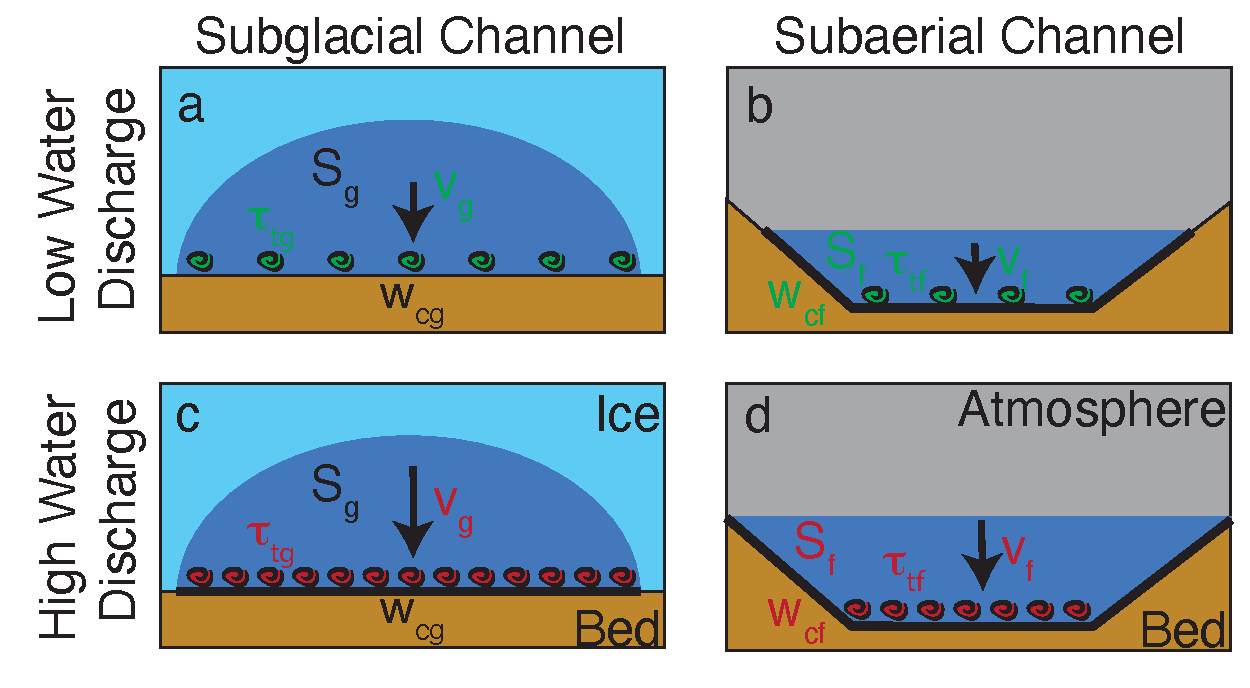
\includegraphics[width=0.8\linewidth]{Fig1.pdf}
    \caption{Sketch for the different responses that subglacial and subaerial channels have to an increase in water discharge.  Water velocity magnitude in the subglacial, $v_g$, and subaerial, $v_f$, channels are shown by arrow length. $S_g$ and $S_f$ represent the wetted area in subglacial and subaerial channels. The subglacial channel widths $w_{cg}$ remain unchanged, while the subaerial channel widths evolve $w_{cf}$. Shear stress $\tau$ is responsible for the mobilization of sediment and increases with the number of makers at the channel bed.
      Note that in the subaerial channel parameterization, channels have rectangular shapes with their width much larger than the depth (Section~\ref{sect:fluv}).}
    \label{fig:cartoon}
  \end{figure}
% \ian{Come back to Daniel's comments}

As a result, sediment mobilization in subaerial and subglacial channels responds differently to changing water discharge.
These differences have been implicitly included in a wide range of available models that  quantify sediment transport from catchments in both subglacial and subaerial channels  \citep[e.g.][]{walder1994,tucker1997,creyts2013,wickert2019,hewitt2019}.
The divergent response of changing water discharge on sediment mobilization capacity may well impact sediment dynamics at glacier margins where flow transitions from pressurized to open channel flow \citep[e.g.][]{lane2016,perolo2018}.
Additionally, the variable response of sediment transport capacity to water discharge in the two systems may affect the interpretation of sediment transport records in glacial systems \citep[e.g.][]{muller1968,richards2003,swift2005,ganti2016}.
Yet, the differing relationship between variations in water discharge and sediment discharge in subglacial and subaerial channels, and implications for sediment discharge records, has been minimally discussed.
Furthermore, thorough observations of water velocity and channel width in subglacial channels are limited and, to these authors' knowledge, not contrasted with subaerial conditions at the glacier margins. %\mauro{self-cite here?}

This manuscript aims to evaluate the relationship between sediment transport capacity and water discharge in subglacial channels, compared to subaerial ones.
In the absence of continuous measurements of subglacial and subaerial water velocity and channel morphology, numerical parameterizations of subglacial and subaerial hydraulics are utilized.
Parameterizations are applied to hydrological records from an Alpine glacier in Switzerland (Fieschergletscher) and  a land-terminating glacier in Greenland (Leverett glacier).
The parameterizations' lumped nature isolates the disparity between water discharge and sediment transport capacity in subglacial systems, independent of the upstream drainage network and sediment access.
Outputs demonstrate differences in the relationships between  water discharge, channel geometry, and water velocity in the subglacial and subaerial channels.
Furthermore, outputs are compared to sediment discharge data from these two catchments.
The manuscript then uses the demonstrated differences between the two channel types to discuss the implications for interpreting the processes driving variability in records of sediment transport from glacierized catchments.

\section{Study sites and data}
\label{sect:ss_data}

Water and suspended sediment data are leveraged from an Alpine and an ice sheet setting.
The Alpine site (\alpine) is  Fieschergletscher in the Swiss Alps ($46^\circ\,29'\,07"$ N, $8^\circ\,08'\,34"$ E).
Water discharge and suspended sediment concentration were collected here at a $1$\unit{min} interval continuously over the period 2014--2021.
See \citet{felix2022} and \citet{felix2021} for more details.

The Leverett Glacier in Greenland (\icesheet) serves as the ice sheet setting.
Water discharge and suspended sediment concentration data were collected roughly $2$\unit{km} downstream from the terminus from June to September 2009 to 2012 ($67^\circ\,03'\,50"$ N, $50^\circ\,12'\,59"$ W).
This data is available from \citet{tedstone2017} at a $5$\unit{min} time interval.
Note that in some cases the removal and relocation of sensors created variations in the sediment concentration not resulting from natural processes.
% was presented in part in \citet{cowton2012} and

\section{Methods}
\label{sect:meth}
The parameterizations below (Sections ~\ref{sect:sub_mode}~and~\ref{sect:fluv}) represent relationships amongst water discharge, water velocity, and channel geometry in both subaerial and subglacial channels (Table \ref{table:vpm}).
Both parameterizations calculate   water velocity, shear stress and width-integrated shear stress, upon which sediment transport depends \citep[Figure \ref{fig:cartoon}; ][]{shields1936}.
The evaluation of these variables omits the selection of a sediment transport relationship and grain-size parameter \citep[e.g.][]{shields1936,meyer1948} needed to calculate sediment transport capacity from shear stress.


\ian{values of f are still high}
\begin{table}[ht]
  \centering
  \caption{Variables, parameters, and constants used in this work. 
    Where two values are given, the first refers to  \alpine{}, a case from Fieschergletscher, and the second to a glacier marginal to the \icesheet{} a case from Leverett Glacier}
  \begin{tabular}{ l  c  c c }
    Name &Symbol&  Value&Units \\ \hline
    \textbf{Variables}  & & & \\
    Water discharge  & $Q$& & $\mathrm{m^{3}\,s^{-1}}$ \\
    Water velocity (glacier, subaerial)  & $v_g,\,v_{f}$& & $\mathrm{m\,s^{-1}}$ \\
    Channel wetted area (glacier, subaerial) &  $S_g, S_f$& & $\mathrm{m^2}$     \\
    Hydraulic diameter &$D_h$&&$\mathrm{m}$\\
    Width of channel floor (glacial, subaerial) & $w_{cg},w_{cf}$&  & $\mathrm{m}$     \\
    Hydraulic head &$\Delta h$&& $\mathrm{m}$\\
    Shear stress (glacier, subaerial) & $\tau_g,\,\tau_f$&& $\mathrm{Pa \, m^{-1}}$ \\
    Width-integrated shear stress (glacier, subaerial) & $\tau_{tg},\, \tau_{tf}$&& $\mathrm{Pa \, m^{-1}}$ \\

         &&&\\

    \textbf{Parameters and Constants}  & & &\\
    Gravitational constant&$g$& $9.81$&$\mathrm{m\,s^{-2}}$\\
    Density of water & $\rho_w$& $1000$ & $\mathrm{kg\,m^{-3}}$ \\
    Density of ice & $\rho_i$& $900$ & $\mathrm{kg\,m^{-3}}$ \\
    Hooke angle of channel & $\beta$ & $\frac{\pi}{2}$ & \unit{rad}\\

    Glacier thickness &$h_{ice}$& $225$ or $700$  &\unit{m}\\
    Effective glacier thickness &$h_o$&$\frac{\rho_i}{\rho_w} h_{ice}$  &\unit{m}\\
    Effective glacier length &$l$&$7000$ or $26,000$&\unit{m}\\
    Constant $1$ in Equation~\ref{eq:dS_dt} &$C_1$&$2.2\times10^{-5}$&\unit{m}$^{-1}$\\
    Constant $2$ in Equation~\ref{eq:dS_dt} &$C_2$&$3.7\times10^{-13}$&\unit{m}$^{-n}\,s^{-1}$\\
    Latent heat of fusion &$L$&$333.5 $&\unit{kJ\,kg}$^{-1}$\\
    Pressure melting coefficient &$c_t$&$7.5\times 10^{-8}$&\unit{K\,Pa}$^{-1}$\\
    Specific heat capacity of water &$c_p$&$4180$&\unit{J\,kg}$^{-1}$\unit{K}$^{-1}$\\

    Ice flow constant &$A$& $5.3\times10^{-24}$ &\unit{Pa}$^{-n}$\,$s^{-1}$\\
    Ice flow exponent &$n$& $3$ &$\mathrm{(-)}$\\
    Friction factor (subglacial) & $f_r$ &$10$ or $20$ & $\mathrm{(-)}$ \\
    Friction factor (subaerial) & $f_p$ & $3$ & $\mathrm{(-)}$\\
    Gradient of channel bed (subaerial) &$\nabla z_c$ &$0.05$& $\mathrm{(-)}$\\
    Subaerial channel factor & $k$ &$3$ or $6.5$ & $\mathrm{s\,m^{-2}}$\\
    Channel geometry exponent &$e$& $\frac{1}{2}$&$\mathrm{(-)}$ \\
    \hline
  \end{tabular}
  \label{table:vpm}


\end{table}

\subsection{Subglacial channel  parameterization}
\label{sect:sub_mode}

To evaluate the shear stress of water flowing across sediments underneath a glacier, the subglacial channel parameterization takes into account the channel geometry and the velocity of the flowing water.
To do this, a modified version of the lumped hydraulics model presented in \citet{clarke1996} and \citet{werder2010} is used.

Here, it is assumed that the water is transported through a subglacial channel flowing down the glacier; \citep[Figure~\ref{fig:cartoon}; ][]{rothlisberger1972}, and that the channel  size responds to frictional heating from water flow and creep closure by ice, using the Darcy-Weisbach formulation for water-flow through a pipe  \citep[e.g.][]{rothlisberger1972,clarke2003}.
The formulation here does not consider the englacial storage of water.
Thus, it is assumed that the changing hydraulic head at the top of the glacier is negligible in the channel size evolution.
The evolution of subglacial channel size $S_g$ is given as
\begin{linenomath*}
  \begin{equation}
    \label{eq:dS_dt}
    \frac{\partial S_g}{\partial t} = C_1 \frac{Q \Delta h}{l} - C_2 \left(h_{o}-\frac{\Delta h}{2}\right)^n\,S_g,
  \end{equation}
\end{linenomath*}
\noindent where $C_1= (1-\rho_wc_pc_t)\,\frac{\rho_wg}{\rho_iL}$ and $C_2=2A(\frac{\rho_wg}{n})^n$ are constants (Table \ref{table:vpm}), $l$ is the length of subglacial channel, $Q$ is water discharge, $\Delta h$ is the hydraulic potential change from the glacier terminus to its top, $h_{o}= \frac{\rho_i}{\rho_w} h_{ice}$ is the ice overburden pressure, and $n$ is Glen's n \citep{glen1955} (usually $n=3$).
The first term on the right side of the equation represents the opening of the channel through frictional heating, while the following term represents the creep closure of the channel from ice deformation.


Following the Darcy-Weisbach, head drop $\Delta h$ is,
\begin{linenomath*}
  \begin{equation}
    \label{eq:dh}
    \Delta h \,  = l \,\frac{1}{g}\,s\,f_r\,\frac{Q^2}{D_h^5}
  \end{equation}
\end{linenomath*}
\noindent where $f_r$ is a friction factor, $D_h$ is the hydraulic diameter, and $l$ is the length overwhich head change occurs. $s$ is a factor accounting for channel geometry \citep{hooke1990}, calculated as:
\begin{equation}
  \label{eq:Hf}
  s = \frac{2\,(\beta -\sin \beta)^2}{(\frac{\beta}{2}\,+\,\sin \frac{\beta}{2})^4},
\end{equation}
where $\beta$ is the central angle of the circular segment that comprises the channel (the so-called Hooke angle). Note that $\beta =\pi$ corresponds to a semi-circle and
smaller values of $\beta$ result in shallow, wide channels.
The hydraulic diameter $D_h$ is converted to wetted area $S_g$ given a channel geometry following \citep{hooke1990}
\begin{equation}
  \label{eq:Dh2S}
  S_g= \frac{D_h^2}{2}\,\frac{(\frac{\beta}{2}+\sin \frac{\beta}{2})^2}{\beta - \sin \beta},
\end{equation}
where $\beta$ is the central angle of the circular segment that comprises the channel (the so-called Hooke angle). Note that $\beta =\pi$ corresponds to a semi-circle and
smaller values of $\beta$ result in shallow, wide channels.


With knowledge of wetted area $S_g$, the shear stress, $\tau_g$, between the water and the channel bed is determined through the Darcy-Weisbach formulation
\begin{equation}
  \label{eq:tau}
  \tau_g=\frac{1}{8}\,f_r\,\rho_w\,v_g^2,
\end{equation}
%
where  the water velocity $v_g = \frac{Q}{S_g}$.

The width of the flat channel floor $w_{cg}$, given angle $\beta$ is
\begin{equation}
  \label{eq:dh2wc}
  w_{cg} = 2  \sin \frac{\beta}{2} \sqrt{\frac{2\, S_g}{\beta -\sin \beta}}.
\end{equation}

The width-integrated shear stress is represented as $\tau_{tg}=w_{cg}\,\tau_g $.

\subsection{Subaerial channel  parameterization}
\label{sect:fluv}

To parameterize the shear stress of water flowing across sediments in the subaerial channel,  the hydraulics parameterization presented in \citet{tucker1997} is implemented.
Using mass conservation and the Darcy-Weisbach relationship as well as assuming that the channel is wide so that the hydraulic radius is well approximated by the flow depth, then
the shear stress $\tau_f$ at the river bed is
\begin{linenomath*}
  \begin{equation}
    \label{eq:DW_tau}
    \tau_f=\frac{\rho_w\,g^{\frac{2}{3}}\,f_p^{\frac{1}{3}}}{2}\, \Big(\frac{Q}{w_{cf}} \Big)^{\frac{2}{3}} \,\nabla z_c^{\frac{2}{3}},
  \end{equation}
\end{linenomath*}
where $\nabla z_c$ is the channel slope, and $f_p$ is the friction factor for subaerial channels.
Channel width $w_{cf}$ is
\begin{equation}
  \label{eq:wcf}
  w_{cf} = k \, Q^\frac{1}{2},
\end{equation}
%
where $k$ is a constant and the exponent is commonly given as $\frac{1}{2}$ \citep{leopold1953}.
%\mauro{This is for so called ``regime channels''}
Water velocity, $v_f$, is given by rearranging Equation \ref{eq:tau} as
\begin{equation}
  \label{eq:vf}
  v_f = \sqrt{\frac{8\,\tau_f}{f_p\,\rho_w}}.
\end{equation}
%
As in Section~\ref{sect:sub_mode}, the width-integrated shear stress is $\tau_{tf}=w_{cf}\,\tau_f$.

\subsection{Implementation}
\label{sect:imp}

The parameterizations above are applied to hydrological records from the Fieschergletscher (\alpine) and the Leverett glacier (\icesheet).
The subglacial and subaerial parameterizations represent the subglacial flow of water exiting a glacier and transitioning to subaerial flow, as it moves through the catchment.
Outputs of the parameterizations are meant to represent generalizable sediment transport characteristics from these hydrographs, rather than actual hydraulic conditions.
To generalize these cases, \alpine{}  is exemplified by relatively thin ice thickness ($h_{ice}$: $225$\,\unit{m}), low water discharge ($\sim\,10$\,\unit{m}$^3$\,\unit{s}$^{-1}$) and high diurnal variability in water discharge (Figure~\ref{fig:model_outs}, a).
\icesheet{}  is exemplified by thick ice  ($h_{ice}$: $700$\,\unit{m}), high water discharge ($\sim\,300$\,\unit{m}$^3$\,\unit{s}$^{-1}$)  and low diurnal variability in water discharge (Figure~\ref{fig:model_outs}, e).

The parameterizations are first applied to a reference test case for each glacier that assumes  subglacial channel with $\beta=\frac{\pi}{2}$ and friction factors $f_r$ and $f_p$ are tuned so that the parameterizations reproduce reasonable velocities for both  the Greenland Ice Sheet and Alpine glaciers \citep[$\sim\,1.6\,$\unit{m}$^3$\,\unit{s}$^{-1}$][]{werder2010b,chandler2013}.
In both subaerial channels, the bed slope, $\nabla z_c$ is $0.05$.
Water velocity, shear stress, and width-integrated shear stress in the subglacial and subaerial channels from this formulation are presented below.

Second, to characterize the variability in sediment discharge capacity in subglacial compared to subaerial channels further, $100$  parameterizations are applied to a range of different channel geometry factors ($\beta$ and $k$) and friction factors ($f_r$ and $f_p$).
Runs with parameter combinations are culled if their mean subglacial water velocity over the season lies outside of the range between $0.75$\,\unit{m}$^3$\,\unit{s}$^{-1}$ and $2$\,\unit{m}$^3$\,\unit{s}$^{-1}$ or if subaerial water velocity lies outside of the range $0.3$\,\unit{m}$^3$\,\unit{s}$^{-1}$ and $1.2$\,\unit{m}$^3$\,\unit{s}$^{-1}$, in accordance with some measurements \citep[e.g.][]{werder2010b,magnusson2012,chandler2013}.
The standard deviation of an output variable over the course of the season is used to quantify the variability of that output.

Lastly,  outputs are compared with the sediment discharge records the glaciers using Spearman rank correlation, or the correlation with respect to the ordering of values from the outputs and observations.
Rank correlation reduces the impact of the non-linear response of sediment transport capacity to the hydrological forcing.
Periods of uncertainty in the data in \icesheet are removed from the analysis.
Outputs and observations are aggregated across timescales from $1$\,\unit{hr} to $15$\,\unit{days} from the $15$\,\unit{min} outputs, by averaging values one half of the timescale before and after a point time.
%\mauro{Here a brief explanation of the rank-stuff would be good.  Also describe the time aggregation.}


\section{Results}

\subsection{Role of water discharge in sediment transport capacity}
\begin{figure}[h]
  \centering
  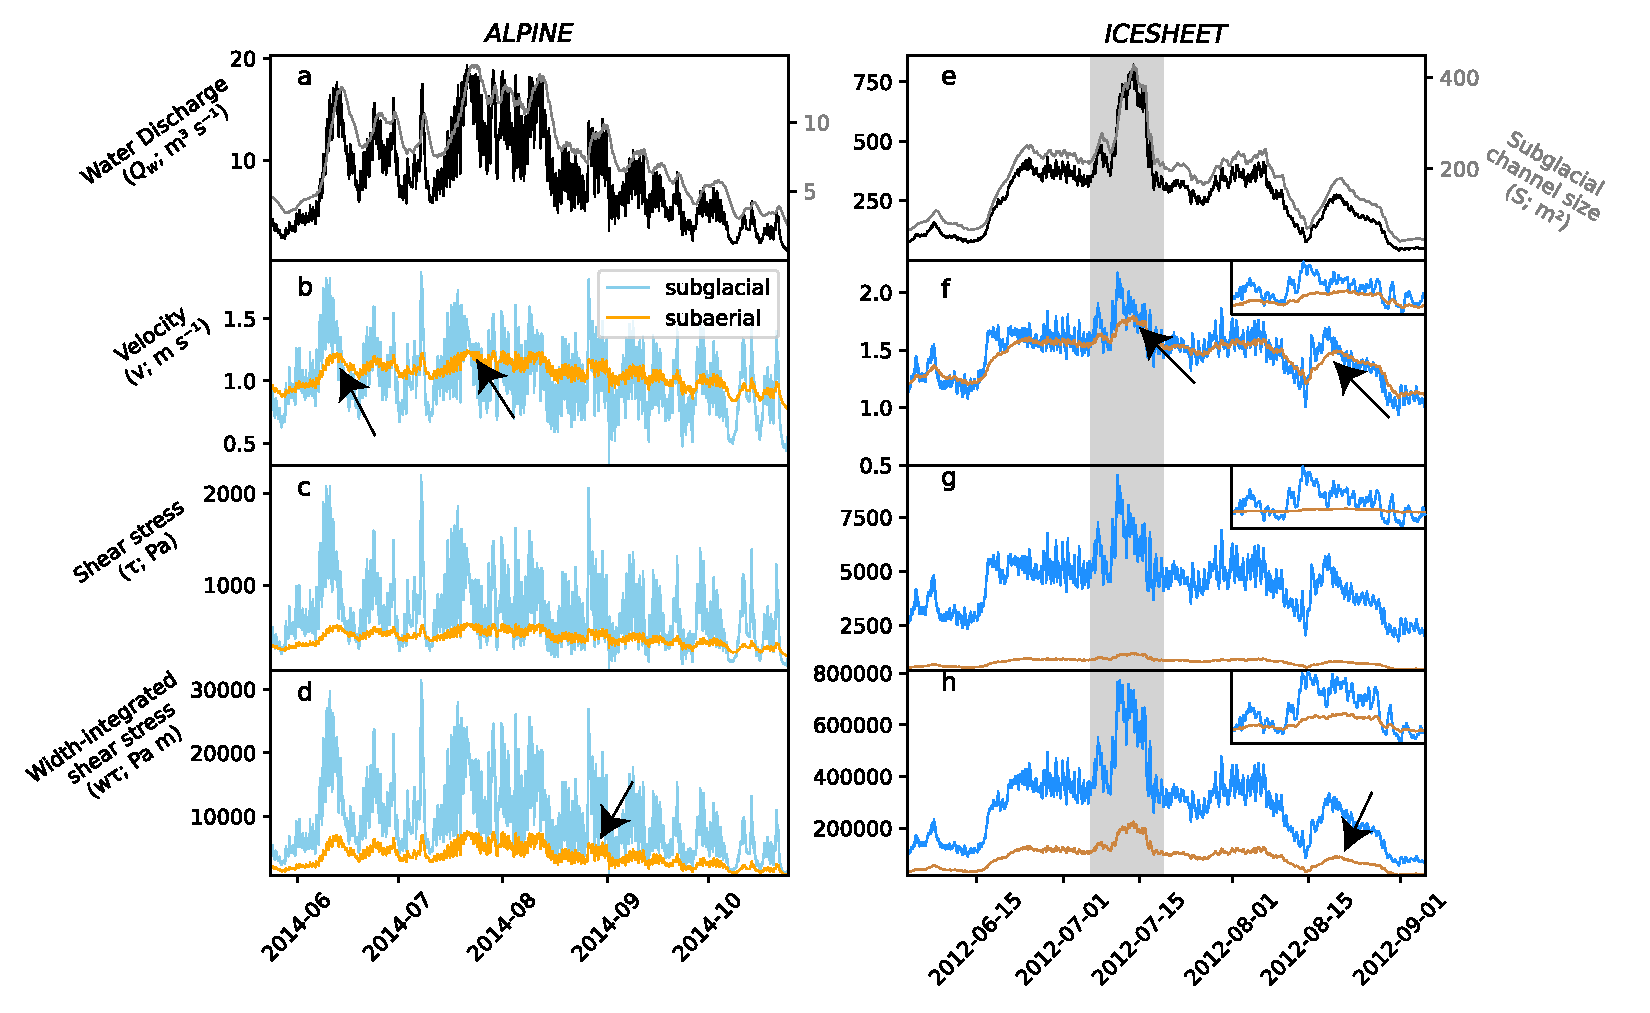
\includegraphics[width=0.9\linewidth]{Fig2.pdf}
  \caption{Parameterization outputs resulting from the hydrographs shown in panels a and e for the cases called \alpine (a-d) and \icesheet{} (e-h). Gray (black) lines in a and e represent the subglacial channel size (water discharge).  In other panels, blue lines represent outputs from the subglacial channel, while orange lines represent the subaerial channel.
    Data in plots are at $15$\unit{min} intervals.
    Arrows denote some events where the variable peaks in the subglacial channel prior to the subaerial one.
    Insets in e-h show the  peak melt event \icesheet{} denoted by the shaded area.
    Note that the x and y axes are different for \alpine{} and \icesheet{} such that they each cover a 
        \ian{NaN values will be removed in final version}
      }
  \label{fig:model_outs}
\end{figure}
Following the parameterizations defined in Sections~\ref{sect:sub_mode}~and~\ref{sect:fluv}, the water velocity, shear stress, and width-integrated shear stress exhibit different seasonal evolutions and peaks. Water velocity and shear stress represent the potential for sediment mobilization, and width-integrated shear stress represents a proxy for the total sediment transport capacity across the channel bed (Figure~\ref{fig:model_outs}).

Over the course of the season, large peaks in water velocity and shear stress, along with width-integrated shear stress, occur in response to increases in water discharge in both \alpine{} and \icesheet{}.
This occurs as the subglacial values are generally larger than the subaerial values, thus more efficient at transporting sediment.
In the subglacial channel, these peaks generally occur over the period when water discharge increases at the fastest rate (Figure~\ref{fig:model_outs}).
Conversely, in the subaerial channel, peaks in these variables occur when water discharge is at its highest value.
As a result, peaks in the subglacial sediment transport variables occur  when the rate of water discharge increase is greatest
is greatest, as opposed to when the maximum amount of water discharge occurs.
The timing of the greatest rate of change in water discharge occurs before the peaks in water discharge.
Here, sediment could be deposited in the proglacial area as the water depressurizes, then remobilized when sediment transport capacity peaks in the subaerial system.

\begin{figure}[h]
  \centering
  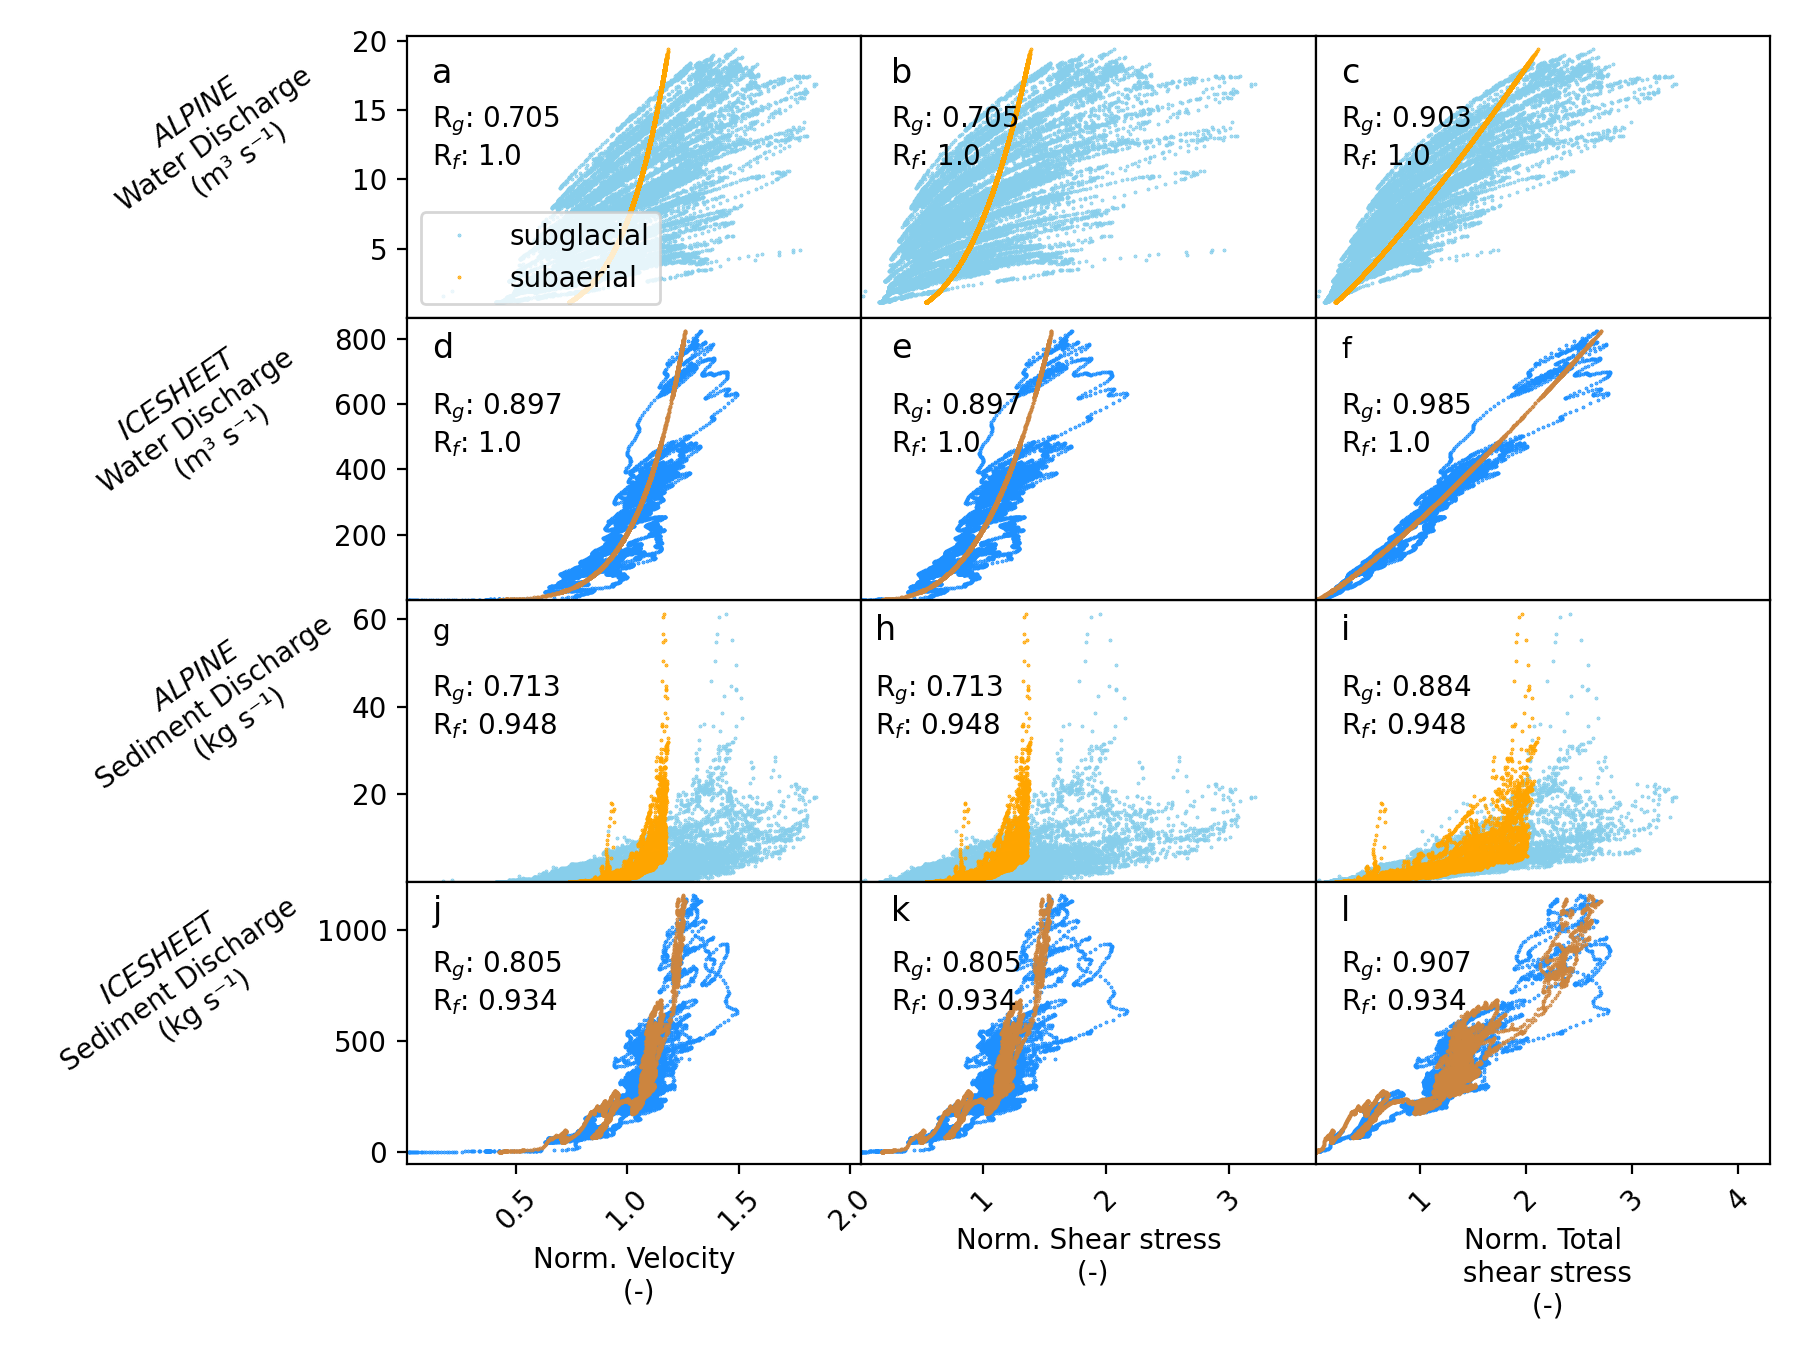
\includegraphics[width=0.9\linewidth]{Fig3.png}
  \caption{Relationship between water discharge and velocity, shear stress, and width-integrated shear stress for \alpine{} (a-c) and \icesheet (d-f).
    These outputs' relationship with measured sediment discharge is given for \alpine in (g-i) and \icesheet (j-l).
    Variables have been normalized to mean values for better comparison amongst the runs.
    $R_g$ ($R_f$) shows the Spearman rank correlation values for the subglacial (subaerial) outputs.
    Plots are shown with data and outputs at $15$\unit{min} interval.
  }
  \label{fig:Qw_vari}
\end{figure}

Each water discharge in the subaerial channel is associated with a single water velocity, shear stress, and width-integrated shear stress, resulting in a perfect rank correlation between the variables (Figure~\ref{fig:Qw_vari} a--f).
Conversely in the subglacial channel,  water velocity, shear stress, and width-integrated shear stress can vary substantially for a given water discharge and width-integrated shear stress varies with respect to the other two  outputs as well (Figure~\ref{fig:Qw_vari} a--f).
For instance, very high values of water velocity and shear stress can occur from minimal water discharge at $2.5$\,\unit{m}$^3$\,\unit{s}$^{-1}$ to the maximum water discharge at over $17$ \,\unit{m}$^3$\,\unit{s}$^{-1}$.
In \icesheet, mean values of water velocity can occur at water discharges between roughly $150$ \,\unit{m}$^3$\,\unit{s}$^{-1}$ and $310$ \,\unit{m}$^3$\,\unit{s}$^{-1}$, effectively spanning much of the water discharge range.

When accounting for the evolving channel width of the subglacial conduit, width-integrated shear stress  across the channel generally increases with water discharge, with improved rank correlation compared to water discharge and water velocity or shear stress (Figure~\ref{fig:Qw_vari} a--f).
Yet even the width-integrated shear stress  can vary substantially, with the highest values occurring at water discharge values ranging from roughly $11$ \,\unit{m}$^3$\,\unit{s}$^{-1}$, to over $17$ \,\unit{m}$^3$\,\unit{s}$^{-1}$.
The variability in width-integrated shear stress is less pronounced in the \icesheet case, in part due to the reduced variability in water discharge.
Yet, a range of width-integrated shear stress can occur at a given discharge (Figure~\ref{fig:Qw_vari} c, f).

\begin{figure}[h]
  \centering
    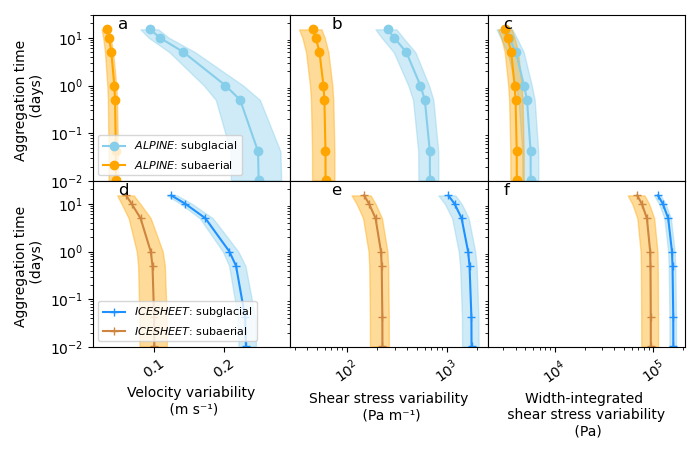
\includegraphics[width=0.9\linewidth]{Fig4.png}
    \caption{Variance (measured by the standard deviation) in water velocity, shear stress, and width integrated shear stress for different time aggregations across the range of subglacial and subaerial channel shapes and friction factors.
      Shaded areas denote the minimum and maximum of the $100$ parameter combinations tested for each of the systems (Section~\ref{sect:imp}).
      Solid lines denote  mean values.
      Top row shows results from \alpine{} case, while bottom row show outputs from \icesheet{} case
      Time intervals shown with markers denote $15$\,\unit{min}, $1$\,\unit{hr}, $12$\,\unit{hr}, $1$\,\unit{d}, $5$\,\unit{d}, $10$\,\unit{d}, and $15$\,\unit{d} aggregation periods.
      Text in columns shows rank correlation between the variable and sediment discharge for the corresponding time period for the subglacial (right column) and subaerial (left column) channels.
      }
    \label{fig:multi_run}
  \end{figure}

The second application examines the impact of a variety of channel shapes and friction factors on the relationship between water discharge and sediment transport capacity, in both systems.
Across the range of parameter values examined, variability in water velocity and shear stress remains higher in the subglacial system compared to the subaerial one.
However, in \alpine{}, the width-integrated shear stress makes the variability between the two systems comparable (Figure~\ref{fig:multi_run}).
Conversely, in \icesheet{}, with lower water discharge variability, the variability in width-integrated shear stress remains higher in the subglacial system across the time aggregation periods.

It is prescient to evaluate the time scales over which the subglacial channels may respond to changing water discharge to understand the influence of variability in sediment transport capacity.
In both cases, the variability in velocity, shear stress, and width-integrated shear stress decrease after $1-5$ day aggregations (Figure~\ref{fig:multi_run}).
This suggests that the effects of the variable response to hydrologic forcing are reduced over longer time aggregations than these.
Yet, substantial differences in variability persist in periods of up to $15$ days, as the variability in aggregations periods longer than this might be conflated with seasonal variations in water discharge.
Note that lags and time of peak sediment transport conditions still occur over these periods (Figure~\ref{fig:model_outs}), while the variability in sediment transport parameters is reduced with increasing time aggregation (Figure~\ref{fig:multi_run}).

\subsection{Relationship between parameterization  outputs and observed sediment discharge}
When comparing the output variables with suspended sediment discharge measurements, velocity, shear stress, and width-integrated shear stress from the subaerial system generally show better correlation with sediment discharge compared to subglacial outputs across the tested subglacial channel parameters (Figures~\ref{fig:Qw_vari} g--l and \ref{fig:multi_run}).
The rank correlation amongst the  subaerial parameterization's three output variables remains fairly constant despite the variable impact of channel shape and consistent scaling with water discharge (Figure \ref{fig:Qw_vari} and Section~\ref{sect:fluv}).
In subglacial channels, velocity and shear stress perform substantially worse in terms of rank correlation with sediment discharge compared to width-integrated shear stress (Figures~ \ref{fig:multi_run}).
In both \alpine{} and \icesheet{}, the  subglacial rank correlation approaches that of subaerial channels over longer time aggregation periods (Figures~ \ref{fig:multi_run}).


\section{Discussion}
\subsection{Context of sediment capacity differences between the channel types}
Quantities that control sediment transport capacity, such as water velocity, shear stress, and width-integrated shear stress, vary differently in response to water discharge in subglacial channels compared to subaerial ones (Figure~\ref{fig:Qw_vari}).
In sediment transport relationships, such as in \citet{meyer1948} or \citet{engelund1967}, that evaluate sediment discharge, shear stress is scaled to the $\frac{3}{2}$ or $\frac{5}{2}$ power, respectively.
The shear stress exponent greater than $1$ magnifies sediment discharge variability beyond the highly variable sediment transport parameters described above (Figure~\ref{fig:multi_run}).
Note that sediment transport relationships describe sediment flux per unit width so that the integrated capacity across channel occurs after application of the exponent, unlike the width-integrated shear stress evaluation here \citep[c.f.][]{tucker1997}.
%Note also that both subglacial and subaerial parameterizations here assume that the distribution of velocity and shear stress is homogeneous across the channel bed, despite the limitations of this assumption \citep[e.g.][]{yager2018}.

The rapid increases and decreases in subglacial sediment transport capacity may compound the variability in sediment transport already present in subaerial systems \citep[Figure~\ref{fig:Qw_vari}; ][]{williams1989,jerolmack2010}.
By applying the discharge - width scaling in Equation~\ref{eq:wcf} to Equation~\ref{eq:v}, by setting $S\, \propto \,Q^{\frac{1}{2}}$, the subaerial channel's width-integrated shear stress response is $\tau_{tf}\, \propto\,  Q$. 
For sufficiently short time periods,  channel width and wetted area are fixed in the subglacial system so that the response of width-integrated shear stress is $ \tau_{tg}\, \propto\,  Q^{2}$, with a larger exponent on $Q$ than in the subaerial case.
As a result, when water discharge fluctuates at shorter timescale than the subglacial channel evolution \citep{gimbert2016}, the width-integrated shear stress varies more with water discharge than in subaerial channels.
Note also that the subglacial shear-stress response to water discharge will be greater than the subaerial's provided that the exponent is less than one in Equation~\ref{eq:wcf}.
However, when subglacial channel size lies in equilibrium with water discharge, the  width-integrated shear stress response is $\tau_{tg}\, \propto \, Q^{\frac{4}{5}}$, similar to subaerial channels.
Hydraulics could trend toward this equilibrium regime after $1-5$ days, when variability in subglacial channels begins to approach that of subaerial channels (Figure~\ref{fig:multi_run}). 
\ian{mauro: should a supplement be made for this? if so, could you send me the one for R-channels? is this essentially equation 14 in werder et al., 2010}

In subglacial channels, peaks occur with the fastest rate of  water discharge increase relative to the channel's growth (Figure~\ref{fig:model_outs}).
In turn, the subglacial channels here contain feedbacks that limit sediment transport capacity as the subglacial channel grows with increasing water discharge capacity, effectively reducing sediment transport capacity with the stabilization of water discharge.
Similar feedback occurs in subaerial systems \citep{phillips2016}, albeit at longer timescales of centuries or more, as opposed to days here \citep{gimbert2016}.

\subsection{Records of sediment discharge  from glaciers}

The increased performance of subaerial hydraulics in representing observations occurs despite the proximity of glaciers to these measurements (Figure~\ref{fig:Qw_vari}).
This could occur for two reasons.

First, these measurement stations are $0.5$ to $2$\,\unit{km} downstream of the glacier terminus \citep{cowton2012,felix2022}, likely a long enough distance for the pressurized subglacial regime to transition to the open channel subaerial one.
The transition of subglacial to subaerial conditions may occur underneath glacier terminus \citep{perolo2018}, especially if closure rates of the ice channels are slow  \citep{rothlisberger1972}.
Furthermore,  if a transport-limited regime persists at the glacier margin, then sediment can be easily mobilized, and subaerial processes could be represented just a short distance downstream.

The consistent relationship between sediment discharge capacity and open channel flow conditions could be pronounced $\sim20$\,\unit{km} downstream of the Leverett site, where a strong correlation persists between sediment plume size and the river's water discharge into the Kangerlussuaq fjord \citep{mcgrath2010}.
In marine-terminating glacier catchments, for contrast, a less consistent relationship may occur between water discharge or melt extent and sediment plume size \citep{tedstone2012}.
Here, ocean water pressurizes subglacial channels at the ice front \citep[e.g.][]{how2017}, so the minimal correlation could result from the inconsistent relationship between subglacial sediment transport capacity and water discharge (Figure~\ref{fig:Qw_vari}). 

Second, the sediment discharge records could represent processes such as increased sediment accessibility when melt extends up glacier, thereby concurrently increasing sediment and water discharge \citep[e.g.][]{vergara2022}.
A supply-limited regime could well persist at many glaciers, because the threshold of motion for sediment can be reached more frequently, and across a range of water discharges, compared to subaerial systems (Figure~\ref{fig:Qw_vari}).
Sediment exhaustion through this process may also explain the stronger dependence of sediment discharge from the Greenland Ice Sheet on basal shear stress, a proxy for bedrock erosion, rather than glacier melt \citep{overeem2017}.
Note that in the data here, however, the absence of lags between the observed sediment and water discharge may suggest that sediment is mobilized close to the measurement stations, as opposed to distal areas of the glacier bed as would be expected in a supply-limited regime \citep[Figure~\ref{fig:model_outs}\, a and e; ][]{williams1989}.

%Regardless of the increased performance of water discharge compared to subglacial sediment transport capacity in the observations, parameterization outputs suggest that additional processes and erosional hiatuses may further complicate signals of sediment discharge from glaciers in response to climate, compared to subaerial systems \citep{jansson2005,ganti2016}.

Sediment discharge records have been used to establish the relationship, or lack thereof, with climate forcing and glacial erosion \citep[e.g.][]{koppes2009a,ganti2016,willenbring2016,mariotti2021}.
The variable relationship between water discharge and subglacial sediment transport capacity presented here mostly applies to the daily- to weekly-time scales controlling the size of subglacial channels (Figure~\ref{fig:multi_run}).
Yet, identifying climatic signals in sediment transport from the transport-limited component of glacier-sedimentary systems may require higher thresholds of water discharge compared to subaerial systems when water discharge is variable  \citep[Figure~\ref{fig:Qw_vari}; ][]{tofelde2021}.

Over time scales longer than days to weeks, the glacier's sediment transport capacity reacts to the ice thickness, controlling the channel closure rate, and the glacier's surface slope, in addition to water discharge \citep[Figure~\ref{fig:multi_run}, ~ Section~\ref{sect:sub_mode}; ][]{rothlisberger1972,shreve1972,stevens2022}.
In a supply-limited state, often assumed in landscape evolution models, then glaciers' sediment discharge record also represents additional processes of sediment availability and bedrock erosion from  water pressure variations and sliding  \citep[e.g.][]{iverson2012,herman2015,delaney2023}.
This multitude of processes lies in contrast to most subaerial systems, where transport capacity typically responds to sediment size, water discharge and hydraulic gradient, and the hydraulic gradient generally remains stable over time scales ranging from years to millennia \citep[Section~\ref{sect:fluv}; e.g.][]{muller1968,whipple1999,wickert2019}.
The stronger link between sediment transport capacity and hydrological forcing in subaerial channels may mean that variations in sediment transport records can be more easily attributed to climatic conditions than in subglacial systems.

\section{Conclusions}

Sediment transport capacity is largely driven by the shear stress of water flowing through a channel and the channel's width.
Subaerial channels  alter their channel width and water velocity immediately in response to changing water discharge.
In contrast, pressurized subglacial channels largely accommodate changing water discharge by altering water velocity and shear stress, upon which sediment transport depends.
Water velocity responds quickly to changes in water discharge because the size of subglacial channels generally evolves slowly compared to variations in water discharge.

Despite these differences, parameterizations of subaerial hydraulics generally demonstrate a better representation of observed sediment discharge variations compared to subglacial channels.
This could be attributed to the role of open channel flow at the glacier margin and in the proglacial area, or the influence of water discharge in driving sediment availability, rather than subglacial sediment discharge capacity.

Implications of the findings here include:
\begin{enumerate}
\item the inconsistent relationship between water discharge and sediment transport capacity underneath glaciers creates increased variability in sediment transport capacity compared to river systems;
\item the timing of peak sediment transport capacity below glaciers generally coincides with large rates of increasing in water discharge, as opposed to the maximum quantity of water discharge;
\item a consistent relationship between water and sediment discharge may represent subglacial sediment access or open channel hydraulics near the glacier margin, instead of subglacial sediment transport capacity.

\end{enumerate}


\section*{Acknowledgments}
\noindent
SNSF Project No. PZ00P2\_202024 provided  funding for I. Delaney.
Code to make the figures, with links to the data, can be found at \url{https://bitbucket.org/IanDelaney/xsection/src/master/}.
Code and data will be uploaded to a permanent repository, with FAIR principles, pending acceptance of the paper.
We thank G. King for commenting on a previous version of this manuscript.



\bibliographystyle{apalike}
\bibliography{PaperLib.bib}




\section{Supplement}



\renewcommand{\figurename}{Figure S}
\setcounter{figure}{0}
\begin{center}
  \begin{figure}[h]
    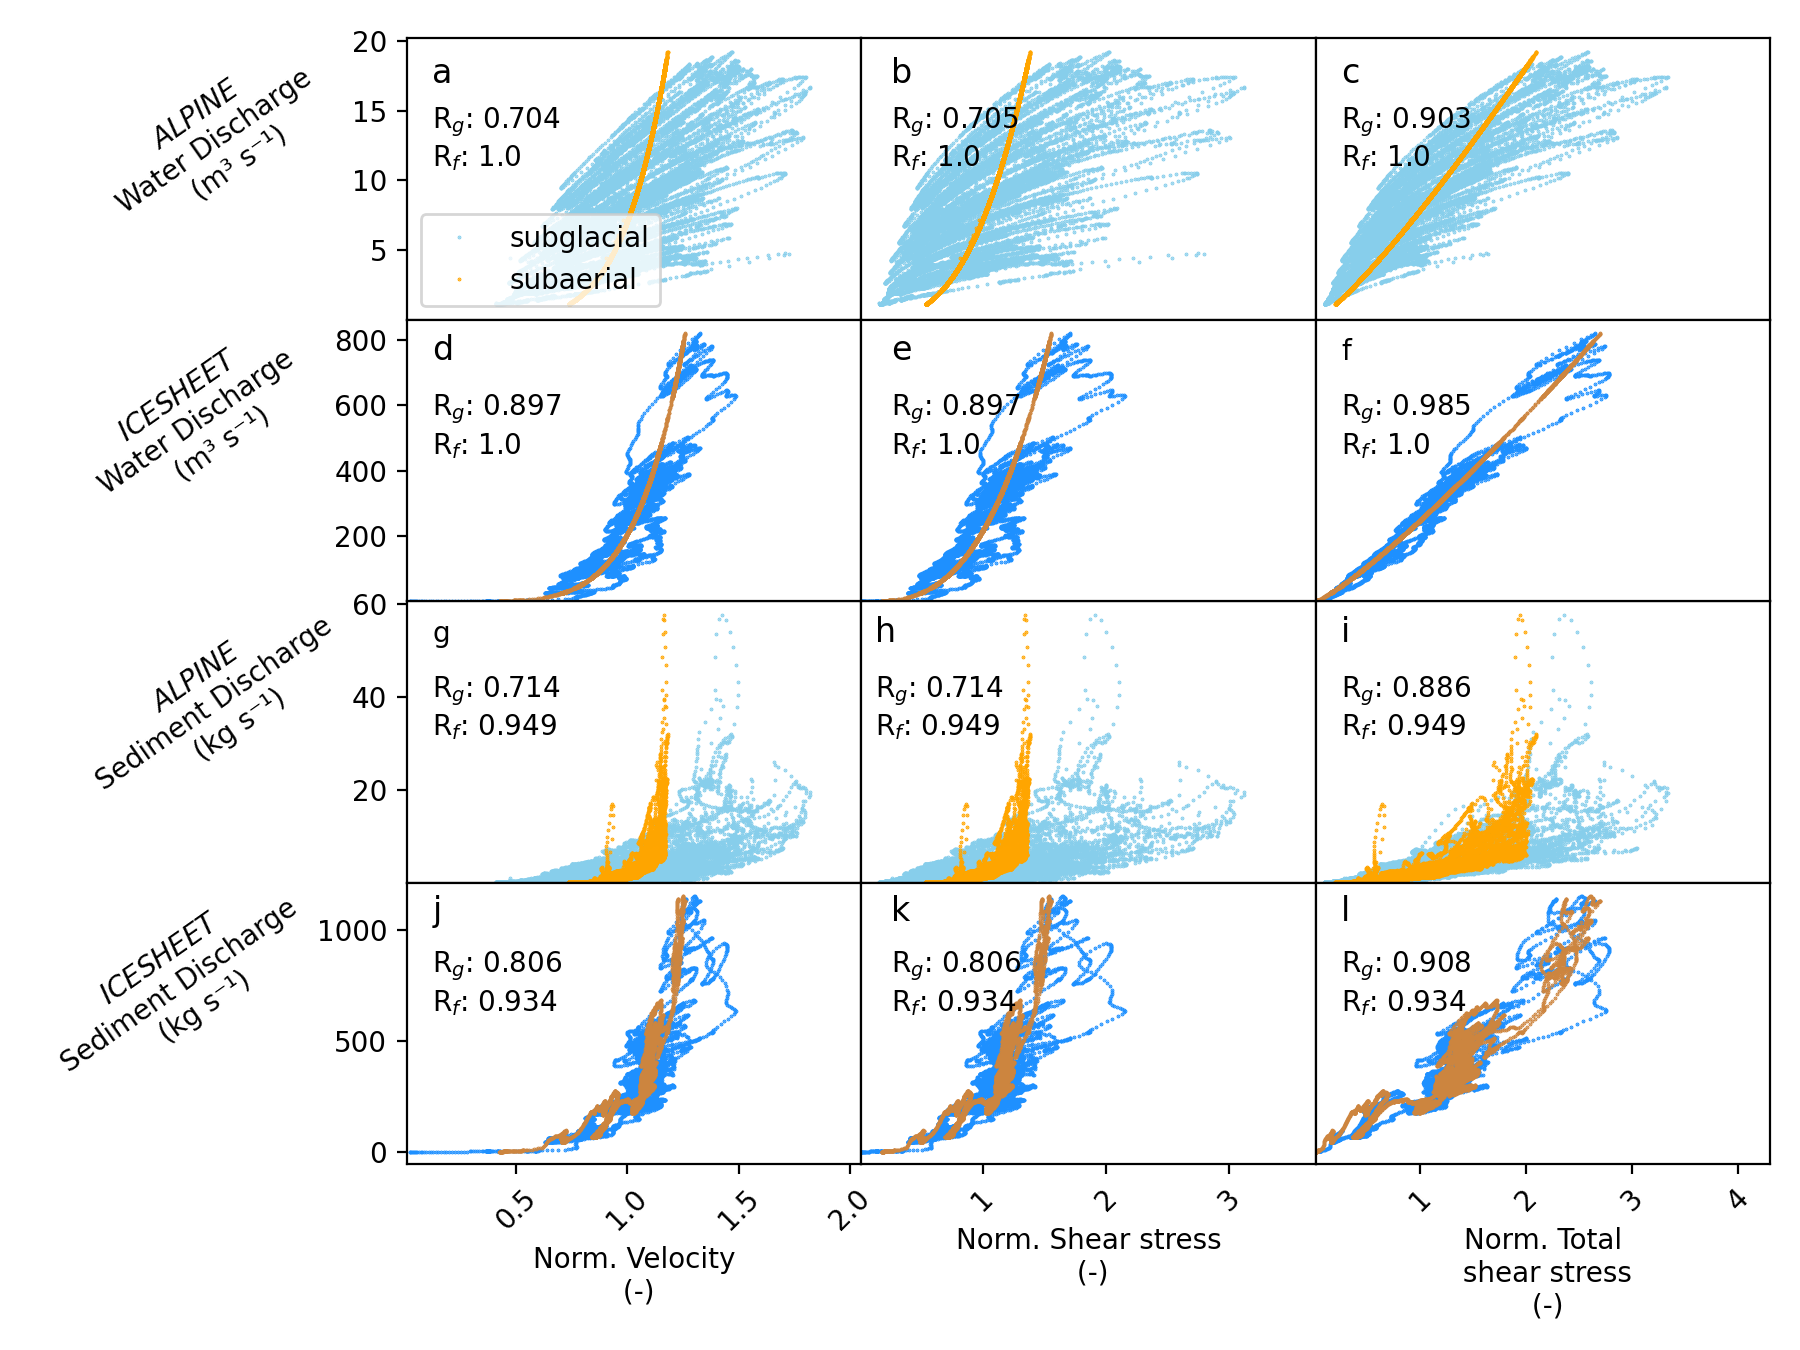
\includegraphics[width=0.7\linewidth]{Fig3_hr.png}
    \caption{As Figure \ref{fig:model_outs}, with $1$ \,\unit{hr} aggregation.}
    \label{fig:model_outs_1hr}
  \end{figure}
\end{center}

\begin{center}
  \begin{figure}[h]
    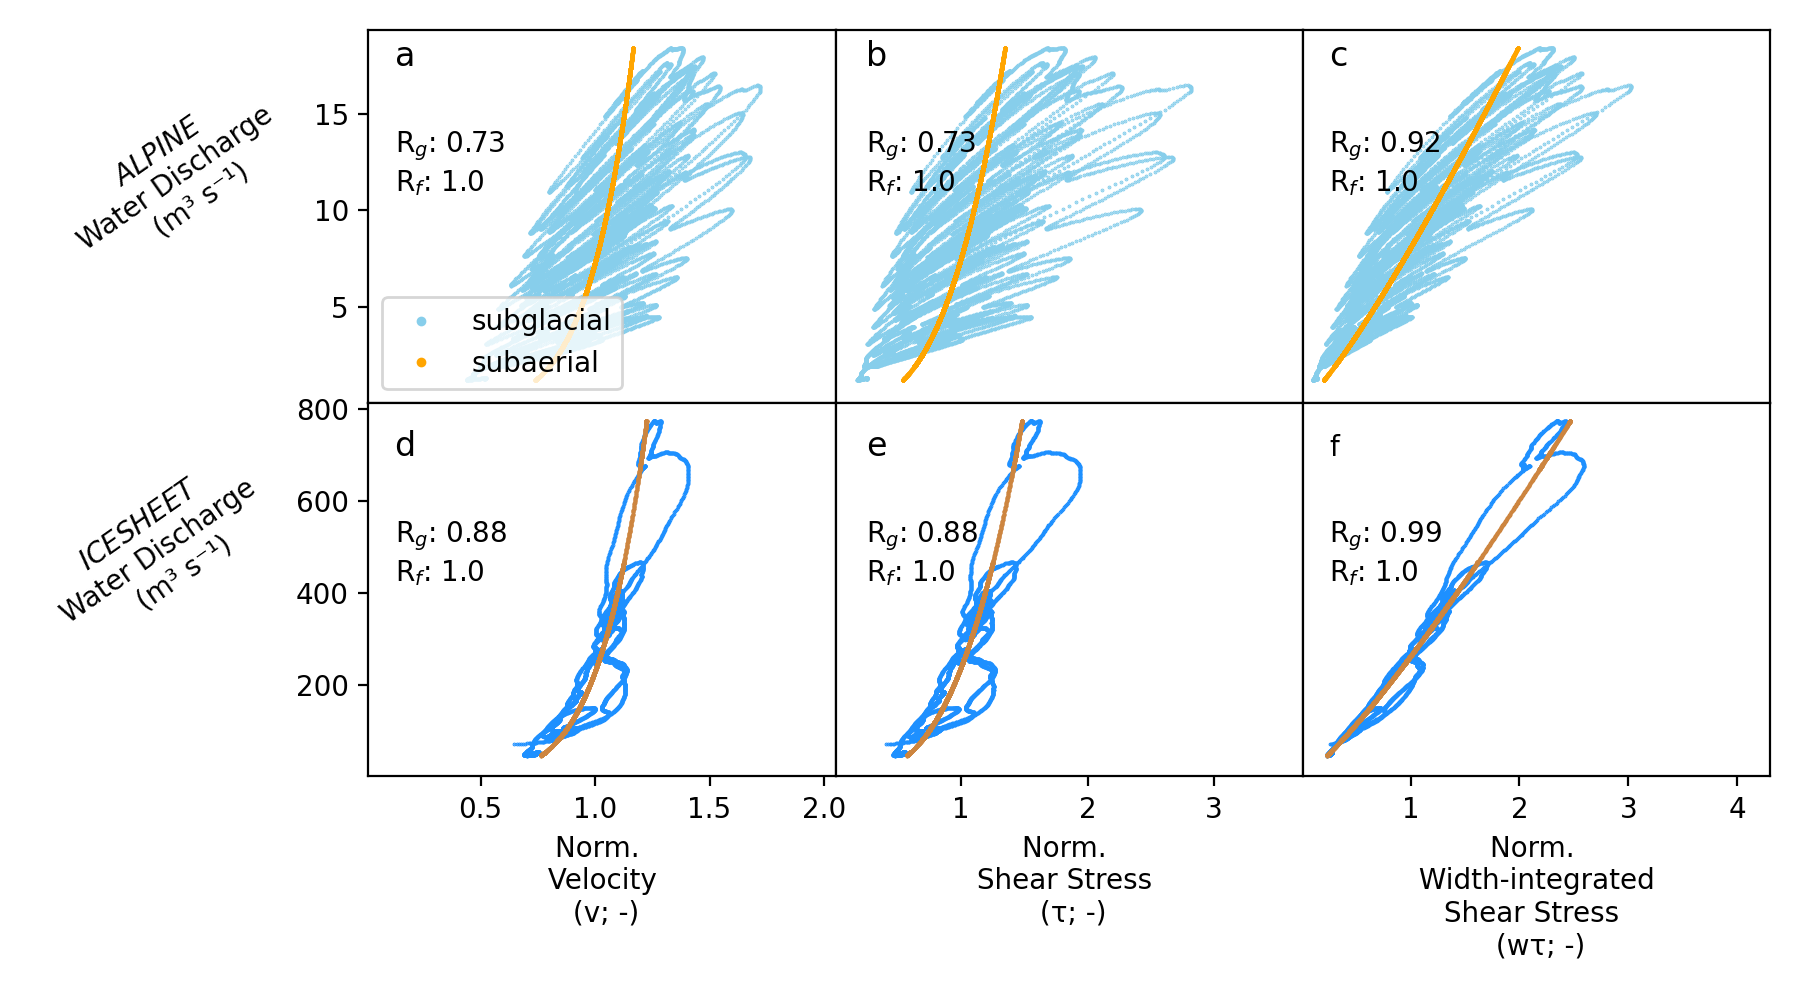
\includegraphics[width=0.7\linewidth]{Fig3_12hr.png}
    \caption{As Figure \ref{fig:model_outs}, with $12$ \,\unit{hr} aggregation.}
    \label{fig:model_outs_12hr}
  \end{figure}
\end{center}


\begin{center}
  \begin{figure}[h]
    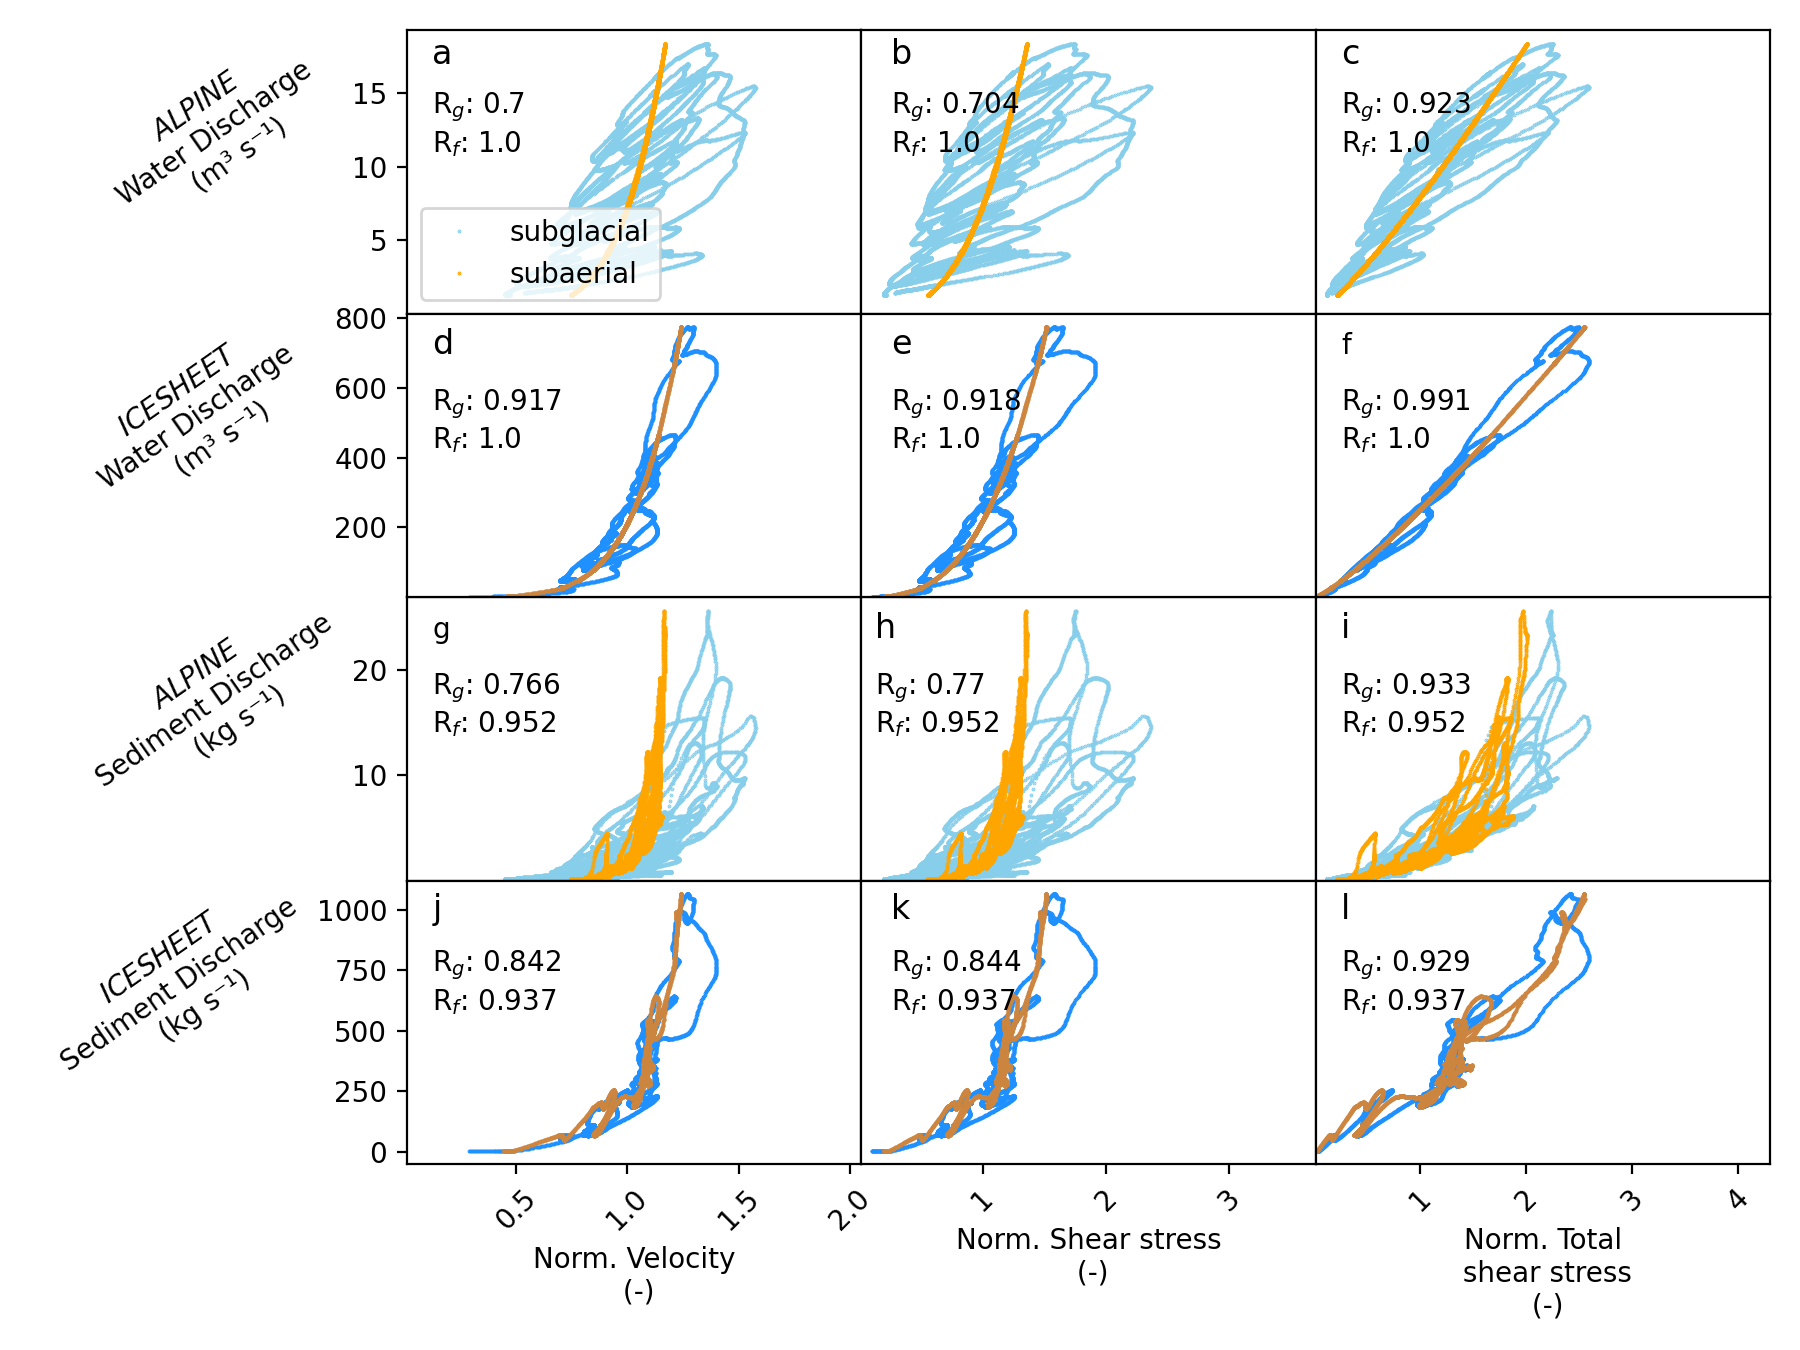
\includegraphics[width=0.7\linewidth]{Fig3_1day.png}
    \caption{As Figure \ref{fig:model_outs}, with $1$ \,\unit{day} aggregation.}
    \label{fig:model_outs_1day}
  \end{figure}
\end{center}


\begin{center}
  \begin{figure}[h]
    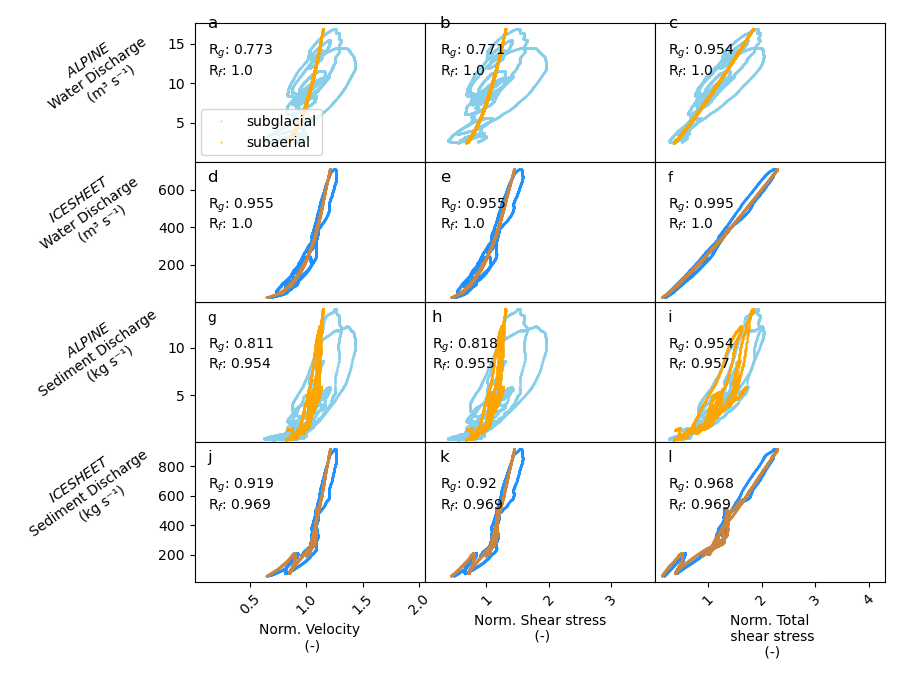
\includegraphics[width=0.7\linewidth]{Fig3_5day.png}
    \caption{As Figure \ref{fig:model_outs}, with $5$ \,\unit{day} aggregation.}
    \label{fig:model_outs_5day}
  \end{figure}
\end{center}

\begin{center}
  \begin{figure}[h]
    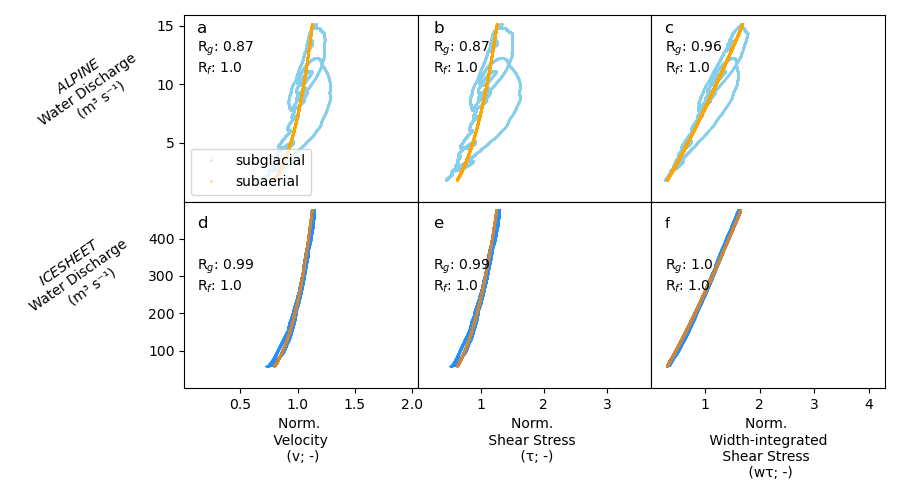
\includegraphics[width=0.7\linewidth]{Fig3_10day.png}
    \caption{As Figure \ref{fig:model_outs}, with $10$ \,\unit{day} aggregation.}
    \label{fig:model_outs_10day}
  \end{figure}
\end{center}
\begin{center}
  \begin{figure}[h]
    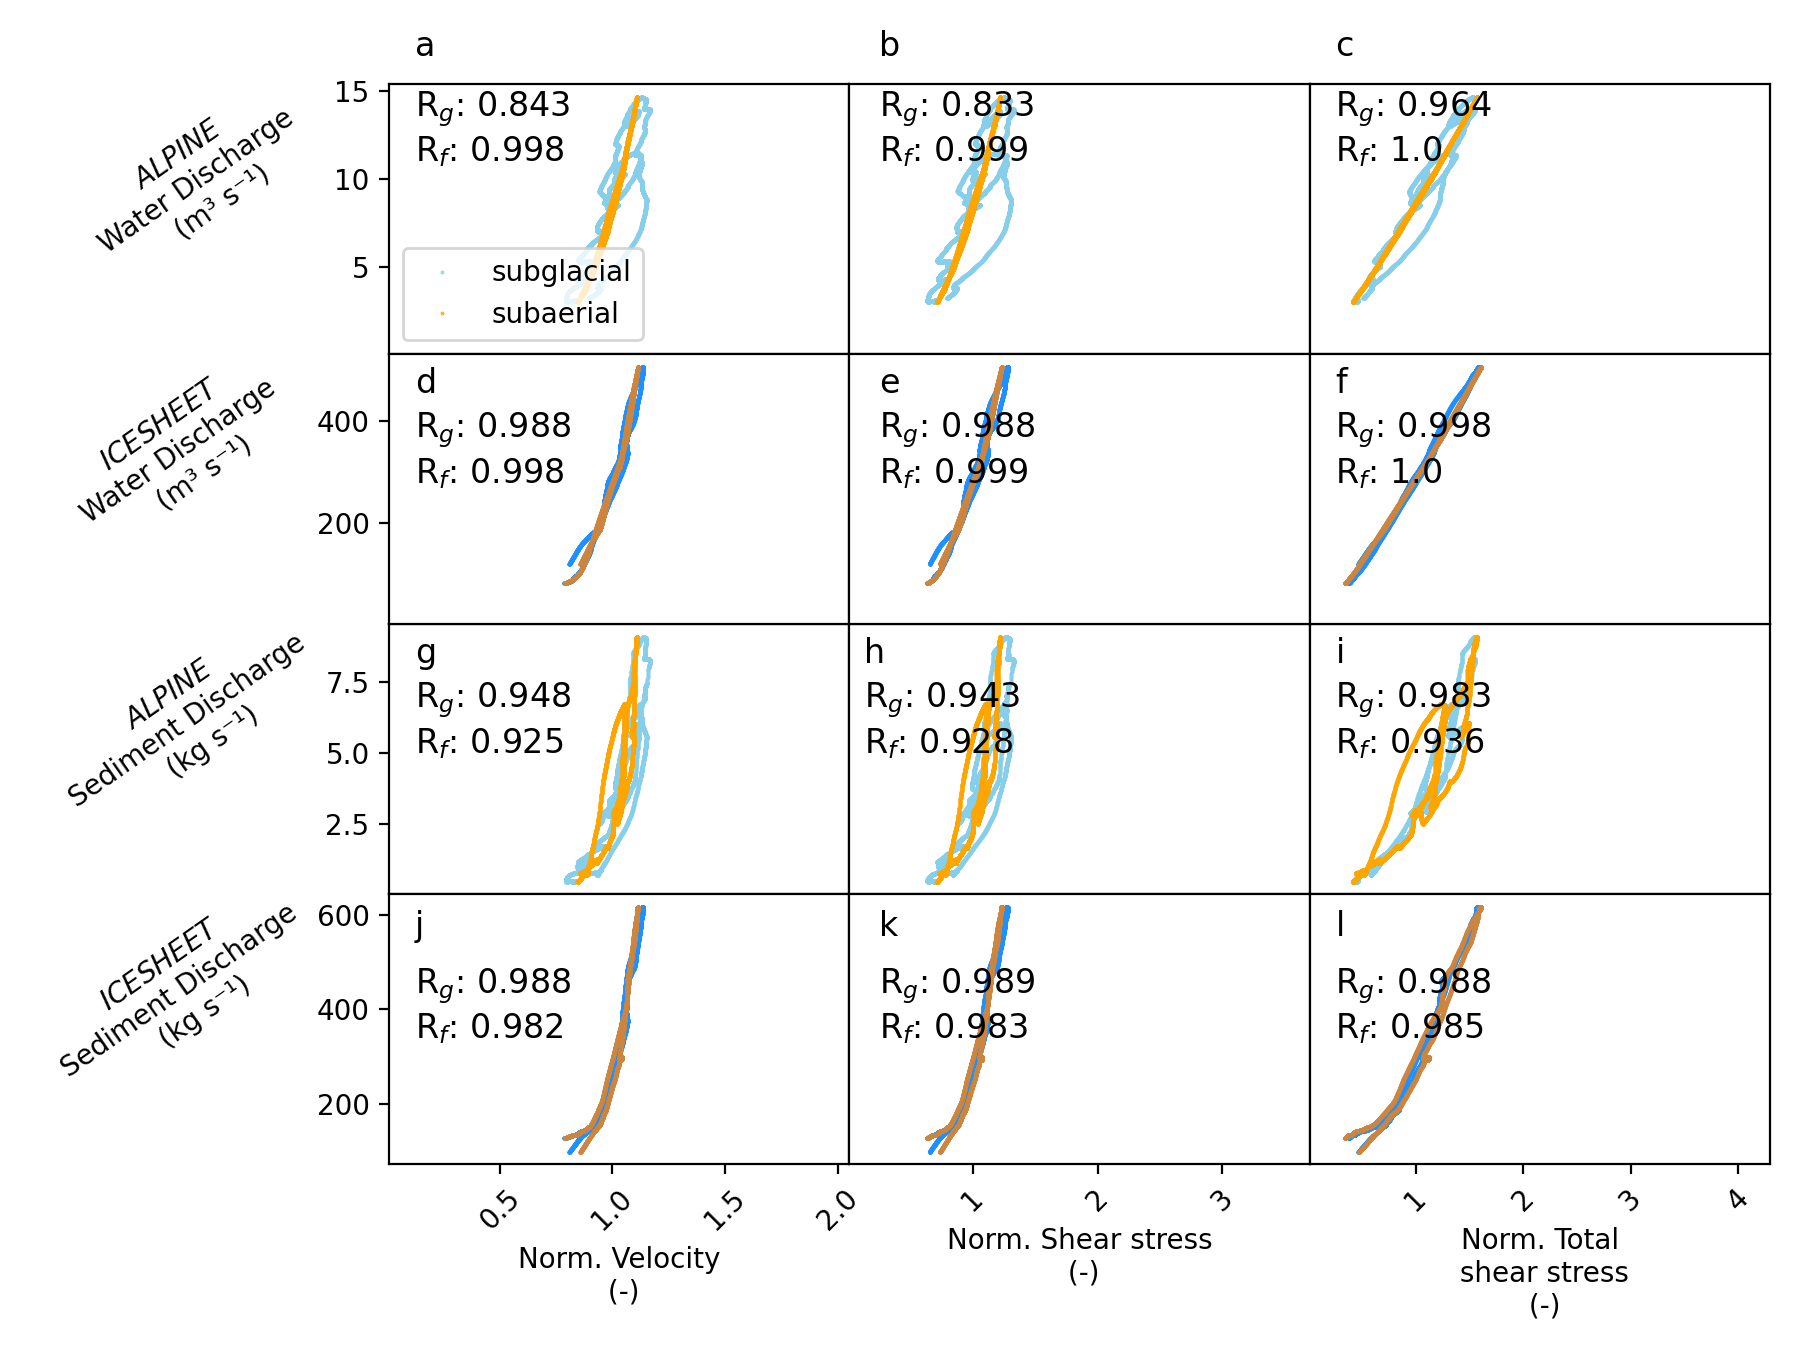
\includegraphics[width=0.7\linewidth]{Fig3_15day.png}
    \caption{As Figure \ref{fig:model_outs}, with $15$ \,\unit{day} aggregation.}
    \label{fig:model_outs_15day}
  \end{figure}
\end{center}

\end{document}

These different characteristics between glacial and subaerial channels show that records of sediment transport downstream of glaciers represent both subglacial and subaerial processes together.
Divergent processes discussed here might be particularly relevant at glacier margins, where water transitions from pressurized subglacial flow to open-channel subaerial flow.
The inconsistent response of sediment transport in subglacial and subaerial systems to changing water discharge could add uncertainty in evaluating  sediment transport signals in subglacial systems.
In addition, the subglacial parameterization shows that sediment transport capacity in glacier systems responds to a large number of factors such as channel size, ice thickness, and glacier surface slope, which may react to climate forcing differently than water discharge alone.


In natural systems, variable mobilization and deposition of sediment occur as water and sediment discharge accumulate as they move through the two-dimensional channel network will compound the already substantial variability in sediment mobilization parameters accounted for here in the lumped parameterization.
Such variability could be especially strong in the subglacial system where meltwater pathways change in response to the evolving hydraulic gradient \citep{delaney2023}.


Results here suggest that increased variability in sediment transport in subglacial systems  could be particularly pronounced on ice sheets with large catchments and reduced water discharge variability over sub-monthly timescales.
Furthermore, width-integrated shear stress across the channel bed can remain relatively high across a range of water discharges (Figures~\ref{fig:model_outs} and \ref{fig:Qw_vari}).
\TODO{is this needed?... does if conflict with observations of the Leverett and not testable}
